\documentclass[border=4pt]{standalone}
\usepackage{tikz}
\usetikzlibrary{positioning, arrows.meta, shapes.geometric, fit, backgrounds, calc}

\begin{document}
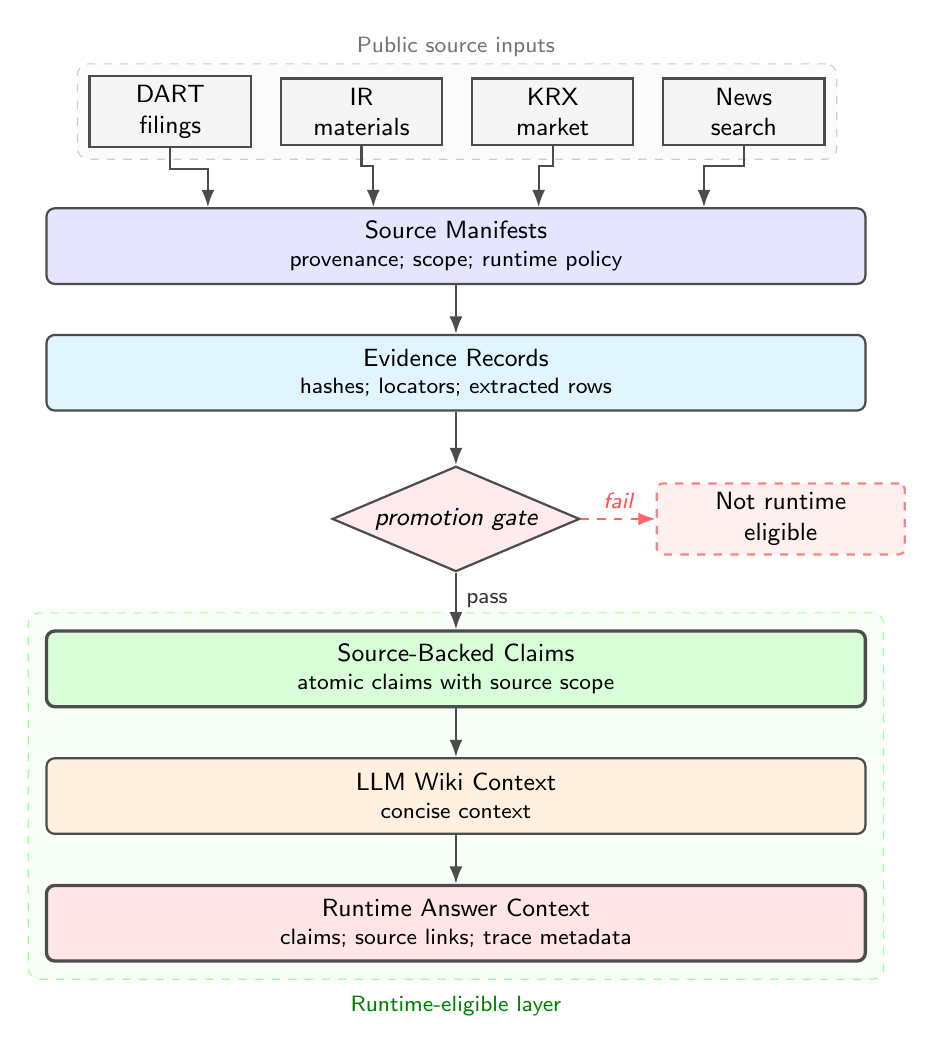
\begin{tikzpicture}[
    font=\small\sffamily,
    node distance=0.62cm,
    stage/.style={
        rectangle, rounded corners=3pt,
        draw=black!70, thick,
        minimum width=10.4cm, minimum height=0.96cm,
        align=center,
        font=\small\sffamily
    },
    rawdoc/.style={
        rectangle, draw=black!70, thick,
        fill=gray!8,
        minimum width=2.05cm, minimum height=0.58cm,
        align=center,
        font=\small\sffamily
    },
    manifest/.style={stage, fill=blue!10},
    evidence/.style={stage, fill=cyan!12},
    claims/.style={stage, draw=black!70, very thick, fill=green!15},
    wiki/.style={stage, fill=orange!12},
    runtime/.style={stage, draw=black!70, very thick, fill=red!10},
    backlog/.style={
        rectangle, rounded corners=2pt,
        draw=red!50, thick, dashed,
        fill=red!6,
        minimum width=3.15cm, minimum height=0.70cm,
        align=center,
        font=\small\sffamily
    },
    gate/.style={
        diamond, aspect=2.35,
        draw=black!70, thick,
        fill=red!8,
        inner sep=1.8pt,
        font=\small\sffamily\itshape
    },
    flow/.style={-{Latex[length=2.2mm]}, thick, draw=black!70},
    rejected/.style={-{Latex[length=2.2mm]}, thick, draw=red!60, dashed},
    label/.style={font=\footnotesize\sffamily, text=black!55},
    arrowlabel/.style={font=\footnotesize\sffamily, text=black!80}
]

% ============ Source inputs ============
\node[rawdoc] (dart) {DART\\filings};
\node[rawdoc, right=0.35cm of dart] (ir) {IR\\materials};
\node[rawdoc, right=0.35cm of ir] (krx) {KRX\\market};
\node[rawdoc, right=0.35cm of krx] (news) {News\\search};
\node[label, above=0.14cm of ir, xshift=1.20cm] {Public source inputs};

% ============ Main pipeline ============
\node[manifest, below=0.78cm of ir, xshift=1.20cm] (manifest) {
    Source Manifests\\[-1pt]
    {\footnotesize provenance; scope; runtime policy}
};
\node[evidence, below=of manifest] (evidence) {
    Evidence Records\\[-1pt]
    {\footnotesize hashes; locators; extracted rows}
};
\node[gate, below=0.68cm of evidence] (gate) {promotion gate};
\node[claims, below=0.72cm of gate] (claims) {
    Source-Backed Claims\\[-1pt]
    {\footnotesize atomic claims with source scope}
};
\node[wiki, below=of claims] (wiki) {
    LLM Wiki Context\\[-1pt]
    {\footnotesize concise context}
};
\node[runtime, below=of wiki] (runtime) {
    Runtime Answer Context\\[-1pt]
    {\footnotesize claims; source links; trace metadata}
};

% ============ Backlog ============
\node[backlog, right=0.95cm of gate] (backlog) {Not runtime\\eligible};

% ============ Arrows from raw sources ============
\draw[flow] (dart.south) -- ++(0,-0.26) -| ([xshift=-3.15cm]manifest.north);
\draw[flow] (ir.south) -- ++(0,-0.26) -| ([xshift=-1.05cm]manifest.north);
\draw[flow] (krx.south) -- ++(0,-0.26) -| ([xshift=1.05cm]manifest.north);
\draw[flow] (news.south) -- ++(0,-0.26) -| ([xshift=3.15cm]manifest.north);

% ============ Main flow ============
\draw[flow] (manifest) -- (evidence);
\draw[flow] (evidence) -- (gate);
\draw[flow] (gate.south) -- node[right, arrowlabel] {pass} (claims.north);
\draw[rejected] (gate.east) -- node[above, font=\footnotesize\sffamily\itshape, text=red!70] {fail} (backlog.west);
\draw[flow] (claims) -- (wiki);
\draw[flow] (wiki) -- (runtime);

% ============ Background grouping ============
\begin{scope}[on background layer]
    \node[fit=(dart)(news), draw=gray!40, dashed, rounded corners, inner sep=4pt, fill=gray!3] {};
    \node[fit=(claims)(wiki)(runtime), draw=green!40, dashed, rounded corners, inner sep=6pt, fill=green!3] (runtimebox) {};
\end{scope}

\node[label, below=0.08cm of runtimebox.south, text=green!50!black] {Runtime-eligible layer};

\end{tikzpicture}
\end{document}
